\section{Analysis using Wensveen's design framework}

Wensveen \cite{Wensveen2004} created a design framework that designers can use to make their product more tangible and interactive. Though his work was already discussed in chapter \ref{chapter: related work}, it is interesting to elaborate on the criteria he has set out and to look at the measure in which the UI design in this project fulfills these criteria.\\

The article states that the key to a more tangible and interactive interaction is by creating a natural coupling between the action that is performed by the user and its associated function in the program through feedback and feed forward. This can be done on six different aspects: time, location, direction, dynamics, expression and modality. A coupling in time can be achieved by having no delay between the action of the user and the feedback of the program. For instance, when pushing a button, it changes color immediately. Location coupling is achieved by placing the feedback for the program in the proximity of the action of the user. In the previous example, the button is coupled in time but also in location because the location where the user pressed is also where the feedback appears. The direction is coupled when the feedback of the program moves in the same direction as the action of the user, such as a scrollbar that moves up when it is dragged up. A coupling in dynamics is achieved by giving feedback with the same position, speed, acceleration and force as the action of the user. For example, when dragging a scrollbar, it follows the cursor with the same acceleration and the same speed so that the relative position of the cursor on the scrollbar doesn't change. Modality is a more abstract term that describes what a user expects to see, feel or hear when a certain action is performed. Wensveen explains modality by giving this example: \emph{the touching of objects can cause a sound or moving an object can be visually perceived}. So to couple action and function, the feedback must react in a way that the user expects it to react based on his experience in the real world. To further clarify this, we present the example of a slide button in an indent. The user expects the button to move within the indent when he drags it, but he also expects it to stop at the end of the indent. The coupling in expression also needs some more clarification. What is meant with a coupling in expression is that the feedback has a metaphorical link to the way the user performs the action or to the function to which the feedback belongs. Wensveen's best example is that of the LED on an Apple Powerbook\textsuperscript{\textregistered}. He states that \emph{the light is an indication of the sleeping state of the system and has the same expression as a relaxed breathing rhythm}. How this is interpreted in this thesis is made clear by the following example. On a Motorola Moto G\textsuperscript{\textregistered} 3rd generation with Android\textsuperscript{\textregistered}, an overview of all the active apps can be shown. To close an app, the user has to swipe it either left or right. The swiping expresses the act of throwing something aside because it is no longer needed which clearly links to the function of closing the app.\\

Each aspect can be coupled through three kinds of feedback or feedforward information: functional, inherent and augmented. Functional information is perceived when the activated function is actually performed. For example, the appearance of the letter \emph{A} when the \emph{A} keyboard button is pressed. Inherent information is feedback inherent to the medium that is used, such as the movement and clicking of a physical keyboard button when it is pressed. The previous examples are all examples of feedback. An example of inherent feedforward is the presence and shape of the \emph{A} key on the keyboard which indicates that it can be pressed. Augmented information is information that is added by the designer and is only bound to the action or function due to the context it appears in. For example, in most operating systems, the progress of moving a file from one drive to another is indicated by a progress bar. This progress bar is not inherent to the function or the medium, it is only bound to the function by the context it appears in.\\

In his article, Wensveen already stated that a NUI, such as designed in this thesis, has almost no inherent information because there is nothing that the designer did not specifically add to inform the user of an action possibility or an action's effect. There is no physical object with which to control the NUI. The only true inherent information on a Kinect is the presence and direction of the camera which indicates that something is registered in that direction. The original article groups all augmented information together to make the link between action and functional information. In this situation, there are two layers of augmented information: the information given by the puppet and the information given by the UI elements such as the rope and the scrollbar. How this works will become clear after the analysis of the puppet and the first UI element. The tool is best used to analyze every action with its respective function separately, but to keep this discussion relatively short only the connections between the user and the puppet, the puppet and the pulling of the rope, the rope and the start of the recording are discussed in detail. The rest is done in more general terms. All links described in the following sections are visualized in figure \ref{puppet_rope_framework}.\\

The coupling between the user and the puppet is crucial because it is the user's way of interacting with other UI elements. If the puppet does not feel natural to the user, the rest of the interaction also feels unnatural. The puppet is coupled to the user in time because there is no delay between the user's movement and the puppet's movement. The hand of the puppet also turns red immediately when the user closes the respective hand. Of course, this is only true when the computer is able to process the information fast enough. This is where the choice for a puppet over a shadow plays a major role, as discussed in chapter \ref{chapter: design}. There is no coupling in location because the puppet is not near the same three-dimensional location as the body of the user. The coupling in direction is strong because the puppet follows every move of the user, though it breaks down when the user tries to reach down below.  The dynamics are coupled very well because the puppet's limbs make the same proportional and relative motion as the user so that the position, acceleration and speed are all proportional to the user's. The link in modality is weaker because there are many situations where the puppet differs from the user's reality, such as the limbs disappearing when the user moves out of the field of vision and the fact that the user cannot feel any of the UI elements that the puppet touches. There is also no expression because there is no metaphorical link between the action of the user and the puppet.\\

%user => puppet => augmented information:
%- time the puppet moves when the user moves with no delay, hand changes color when closed
%- no location the puppet's hand is not near the same three dimensional location as the hand of the user
%- direction the puppet's limbs move in is the same direction as the user, the only exception is when the user tries to bend down.
%- dynamics the puppet's limbs are make the same proportional and relative movements as the user so the position, acceleration and speed are all proportional.
%- no modality there are to many things that differ from reality such as limbs disappearing when they are out of the camera's field of view and limbs go over all of the UI objects
%- no expression there is no metaphorical link between the action of the user and the puppet.

The rest of the UI elements only interact with the puppet. They are represented in figure \ref{puppet_rope_framework} as the second augmented information block. The rope, as seen in figure \ref{rope handle reaction}, to start a recording is coupled to the puppet in time because it changes color and moves only when the puppet touches it. It is also coupled in location because it only changes around where the hand of the puppet is located. The coupling in both direction and dynamics is apparent because the rope moves downward with a downward move of the hand at the same acceleration and speed. Besides the fact that the rope can be grabbed like a real-life rope, the coupling in modality is weak because it doesn't react to the user's touch with the same physics that a rope would. There is no link in expression because it doesn't matter how the puppet pulls the rope. The effect is always the same.\\

%Puppet => rope for recording :
%- time it changes color or moves when the puppet touches it
%- location it changes color around where the hand touches the UI_element
%- direction it moves in the same direction as the hand of the puppet when grabbed
%- dynamics are coupled with those of the puppet because the element is fixed to the hand of the puppet.
%- no modality coupling is present, the rope only goes down for any other movement it does not react like a rope should
%- expression it turns red when grabbed, red is generally a signaling color 

The activated function, i.e.\ starting the recording, is only coupled in time with the rope UI element because it doesn't matter where, in which direction or with what speed the user pulls the rope. It always results in the recording window appearing. There is however a more direct coupling between this function and the puppet: the record window appears on the location of the puppet.

\begin{figure}[H]
	\begin{center}
		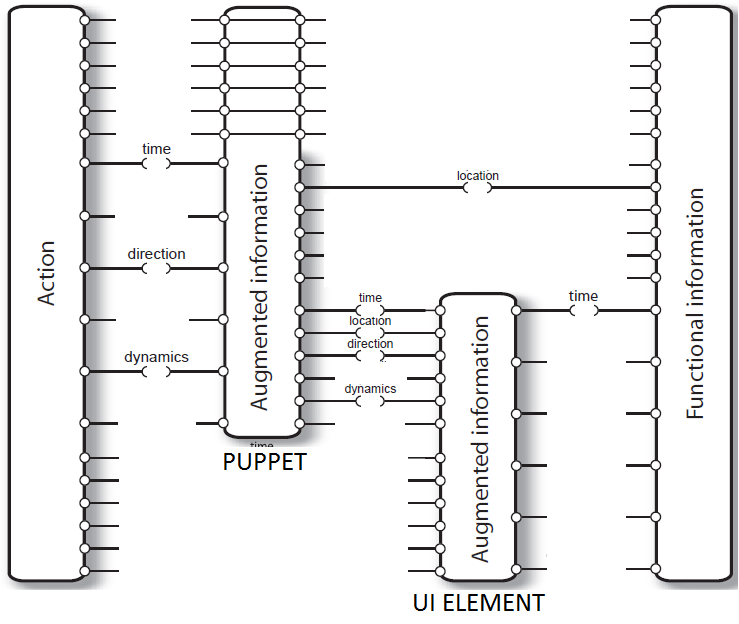
\includegraphics[width=14cm]{figures/standard_framework_Rope.png}
		\caption{\emph{Overview of the framework couplings for the puppet and the rope UI element}}
		\label{puppet_rope_framework}
	\end{center}
\end{figure}

The links from the user to the puppet stay the same for all of the UI elements. Links from puppet to UI element or function can be different. Assuming the computer can handle the workload, most of the UI elements are coupled in time with the puppet. A notable instance of time coupling is when the user wants to replay a recording, as seen in figure \ref{replay of element six}. Only when the puppet's hand hovers over the recording in the selection box area the recording starts to play. The change to green of the selection box is coupled to the puppet's hand in location. It makes the bridge to the replay screen because it also changes to green at the same time. The number of the recording is also shown on the screen at that time. The thorough link in time is because the coupling in location is so weak as mentioned before and no other couplings can be made. Both the scrolling and the delete slide have the same location, direction and dynamic coupling as the rope due to the general color coding and the fact that the movement of the UI elements are always the same as that of the hand that acts upon it. Though the delete action, seen in figure \ref{delete functionality}, has a special expression between the UI element and its function, the red color refers to signals like a red traffic sign or red traffic light that demand attention because they contain important information. 

%rope => open record screen
%- time it appears when the rope is pulled
%- no other links
%
%puppet => record screen 
%- location link the screen is drawn were the puppet stands.
%
%start recording
%
%end recording
%
%replay recordin
%- time has a strong link it only plays when the user hovers over it, same color, same number, 
%- location doesn't have a link it is far away
%- dynamics not really a link
%- no expression
%- no modality
%
%- 
%
%start scrolling
%- time when the puppet hoverover it green
%- location same time
%- direction follows hand
%- dynamics same dynamics as the hand
%-  no modality
%- no expression
%
%end scrolling 
%
%puppet => delete
%- time no delay
%- location hand over the middle of the object
%- direction follows hand 
%- no modality
%- red expression, delete fills with red expressing 
%
%
%
%
%link action to function: eloborate on what this means
%6 aspects that can do this: explain the exact meaning
%each aspect can have feedback and feedforward in 3 ways functional, augmented, inherent. give examples
%talk about the NUI only augmented feedback
%then talk about were our connection lay. and the reason why they are connected
